\section{\textsc{Salatsauce mit Kräutern}}

\subsection*{Zutaten für 100ml:}

\begin{tabular}{p{7.5cm} p{7.5cm}}
	& \\
	40ml Essig & Kräuter \\
	60ml Öl & Schalotten \\
	Salz \& Pfeffer &
\end{tabular}

\subsection*{Serviervorschlag:}

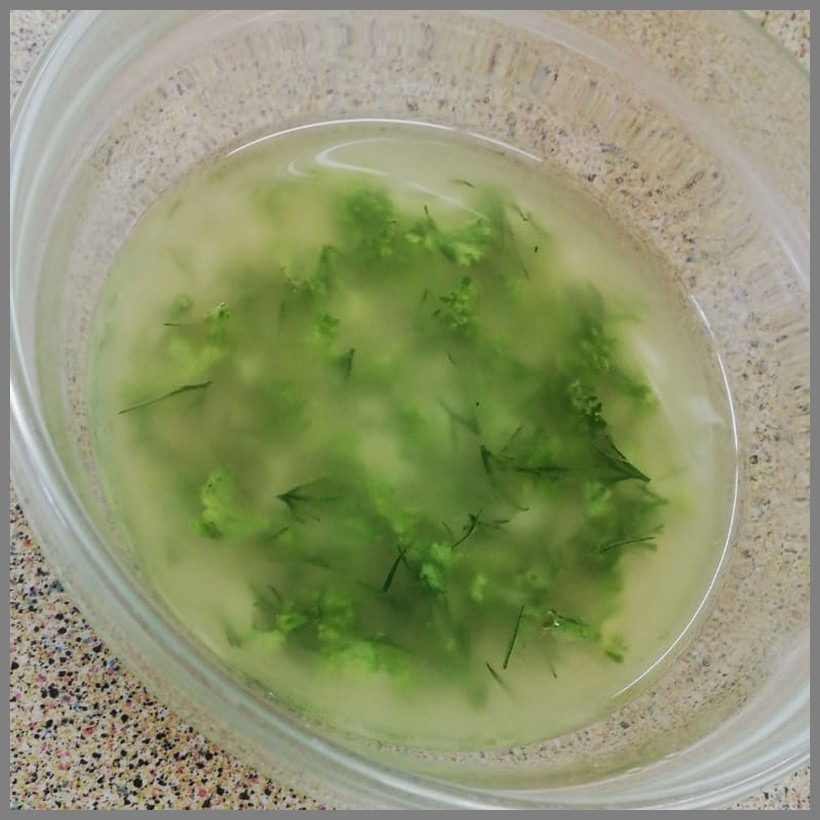
\includegraphics[width=\textwidth]{img/d_krauter.jpeg} \cite{dkrauter}

\subsection*{So geht's:}

\begin{tabular}{p{15cm}}
	\\
	Salz in Essig auflösen, Öl einrühren und anschliessend würzen.\\
	Frisch gehackte Kräuter und fein geschnittene Scharlotten dazugeben.\\
	\\
	Geeignet zu Salaten ohne Obst.
\end{tabular}
